%%%%%%%%%%%%%%%%%%%%%%%%%%%%%%%%%%%%%%%%%%%%%%%%%%%%%%%%%%%%%%%%
%%%%%%%%%%%%%%%%%%%%%%%%%%%%%%%%%%%%%%%%%%%%%%%%%%%%%%%%%%%%%%%%
%%%%
%%%% This text file is part of the source of 
%%%% `Introduction to High-Performance Scientific Computing'
%%%% by Victor Eijkhout, copyright 2012-8
%%%%
%%%% This book is distributed under a Creative Commons Attribution 3.0
%%%% Unported (CC BY 3.0) license and made possible by funding from
%%%% The Saylor Foundation \url{http://www.saylor.org}.
%%%%
%%%%
%%%%%%%%%%%%%%%%%%%%%%%%%%%%%%%%%%%%%%%%%%%%%%%%%%%%%%%%%%%%%%%%
%%%%%%%%%%%%%%%%%%%%%%%%%%%%%%%%%%%%%%%%%%%%%%%%%%%%%%%%%%%%%%%%

Another important topic in high performance computers is their power
consumption. Here
we need to distinguish between the power consumption of a single
processor chip, and that of a complete cluster.

As the number of components on a chip grows, its power consumption
would also grow. Fortunately, in a counter acting trend,
miniaturization of the chip features has simultaneously been reducing
the necessary power. Suppose that the feature size~$\lambda$ (think:
thickness of wires) is scaled down to $s\lambda$ with~$s<1$. In order
to keep the electric field in the transistor constant, the length and
width of the channel, the oxide thickness, substrate concentration
density and the operating voltage are all scaled by the same factor.

\Level 1 {Derivation of scaling properties}

The properties of \emph{constant field scaling}\index{field scaling} or
\indexterm{Dennard scaling}~\cite{Bohr:30yearDennard,Dennard:scaling}
are an ideal-case description of the properties of a circuit
as it is miniaturized. One important result is that power density 
stays constant as chip features get smaller, and the frequency 
is simultaneously increased. 

The basic properties derived from circuit theory are that,
if we scale feature size down by~$s$:
\[
\begin{array}{|l|c|}\hline
\hbox{Feature size}&\sim s\\
\hbox{Voltage}&\sim s\\
\hbox{Current}&\sim s \\ 
\hbox{Frequency}&\sim s\\
\hline
\end{array}
\]

Then we can derive that 
\[ \hbox{Power} = V\cdot I \sim s^2, \]
and because the total size of the circuit also goes down with~$s^2$,
the power density stays the same.
Thus, it also becomes possible to
put more transistors on a circuit, and essentially not change the cooling
problem.

This result can be considered
the driving force behind \indexterm{Moore's law},
which states that the number of transistors in a processor
doubles every 18 months.

The frequency-dependent part of the power a processor needs
comes from charging and discharging the capacitance of the circuit, so
\begin{equation}
\begin{array}{|l|l|} \hline
\hbox{Charge}&q=CV\\
\hbox{Work}&W=qV=CV^2\\
\hbox{Power}&W/\hbox{time}=WF=CV^2F \\ \hline
\end{array}
\label{eq:power}
\end{equation}
This analysis can be used to justify the introduction of multicore processors.

\Level 1 {Multicore}

At the time of this writing (circa~2010), miniaturization of
components has almost come to a standstill, because further lowering
of the voltage would give prohibitive leakage. Conversely, the
frequency can not be scaled up since this would raise the heat
production of the chip too far. 
%
\begin{figure}[ht]
  \begin{quote}
  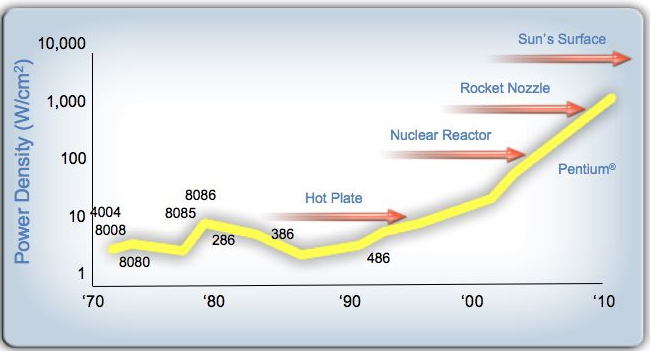
\includegraphics[scale=.6]{graphics/chipheat0}
  \end{quote}
  \caption{Projected heat dissipation of a CPU if trends had
    continued -- this graph courtesy Pat Helsinger}
  \label{fig:chipheat}
\end{figure}
%
Figure~\ref{fig:chipheat} gives a dramatic illustration of the heat
that a chip would give off, if single-processor trends had
continued.

One conclusion is that computer design
is running into a \indextermbus{power}{wall}, where the sophistication
of a single core can not be increased any further (so we can for
instance no longer increase \indexac{ILP} and
\indextermbus{pipeline}{depth}) and the only way to increase
performance is to increase the amount of explicitly visible
parallelism. This development has led to the current generation of
\indexterm{multicore} processors; see section~\ref{sec:multicore}. It
is also the reason \acp{GPU} with their simplified processor design
and hence lower energy consumption
are attractive; the same holds for \acp{FPGA}.
One solution to the power wall problem is introduction
of \emph{multicore}\index{multicore!motivated by power} processors.
Recall equation~\ref{eq:power}, and compare a single processor to two 
processors at half the frequency. That should have the same computing power, right?
Since we lowered the frequency, we can lower the voltage if we stay with the same 
process technology.

The total electric power for the two processors (cores) is, ideally,
\[ \left.
\begin{array}{c}
C_{\mathrm{multi}} = 2C\\
F_{\mathrm{multi}} = F/2\\
V_{\mathrm{multi}} = V/2\\
\end{array}\right\} \Rightarrow
P_{\mathrm{multi}} = P/4.
\]
In practice the capacitance will go up by a little over~2, and the
voltage can not quite be dropped by~2, so it is more likely that
$P_{\mathrm{multi}} \approx 0.4\times
P$~\cite{Chandrakasa:transformations}.  Of course the integration
aspects are a little more complicated in
practice~\cite{Bohr:ISSCC2009}; the important conclusion is that now,
in order to lower the power (or, conversely, to allow further increase
in performance while keeping the power constant) we now have to start
programming in parallel.

\Level 1 {Total computer power}

The total power consumption of a parallel computer is determined by
the consumption per processor and the number of processors in the full
machine. At present, this is commonly several Megawatts. By the above
reasoning, the increase in power needed from increasing the number of
processors can no longer be offset by more power-effective processors,
so power is becoming the overriding consideration as parallel
computers move from the petascale (attained in 2008 by the
\indextermbus{IBM}{Roadrunner}) to a projected exascale.

In the most recent generations of processors, power is becoming an
overriding consideration, with influence in unlikely places. For
instance, the \ac{SIMD} design of processors (see
section~\ref{sec:simd}, in particular section~\ref{sec:sse-avx}) is
dictated by the power cost of instruction decoding.

\endinput

\Level 1 {Frequency scaling}

For the Xeon Scalable Processors (Skylake Xeon), the core frequency is
governed by
(1) The number of active cores
(2) The width of the SIMD units that are active
(3) The power consumption of the package
(4) The temperature of the package

The first two items determine the maximum frequency of the cores from
a table lookup, while the last two items can reduce the frequency to
avoid violating power or temperature limits.

The frequencies are all documented in Figures 1-15 of the document
``Intel Xeon Processor Scalable Family Specification Update''
(336065-005, February 2018).

Figures 4-6 show the maximum core frequency for the Xeon Platinum 8160
processors as a function of SIMD width (not precisely, but this is how
the tables are organized -- see more details at the bottom of this
note) and number of cores used.
For all cores in use, each the base & maximum frequencies (GHz) for
the three SIMD widths are:
non-AVX 2.1 2.8
AVX256 1.8 2.5
AVX512 1.4 2.0

Figures 1-3 show the maximum core frequency for the Xeon Gold 6148
processors as a function of SIMD width and number of cores used.
For all cores in use, each the base & maximum frequencies (GHz) for
the three SIMD widths are:
non-AVX 2.4 3.1 ``level 0 turbo license'' -- see notes at bottom
AVX256 1.9 2.6 ``level 1 turbo license'' -- see notes at bottom
AVX512 1.6 2.2 ``level 2 turbo license'' -- see notes at bottom

Based on these tables, your observations of average frequency are all
consistent with the expected behavior.

Both the Xeon Platinum 8160 and Xeon Gold 6148 have a power limit of
150 Watts, so it is certainly possible that the 4 extra cores on the
Xeon Platinum 8160 in Stampede2 are causing more significant frequency
reductions due to hitting the power limit. (Stampede2 is very well
cooled, so it is extremely unlikely that you are hitting temperature
limits.)

Since the upgrade to CentOS 7.6 in February, the ``perf stat'' command
has the ability to read the package energy counters on the compute
nodes.
An example using the STREAM benchmark:

perf stat -a -A -e ``power/energy-pkg/''
./stream.COMMON-AVX512.80M.1000x

gives the output:

-------------------------------------------------------------
Array size = 80000000 (elements), Offset = 0 (elements)
Memory per array = 610.4 MiB (= 0.6 GiB).
Total memory required = 1831.1 MiB (= 1.8 GiB).
-------------------------------------------------------------
Function Best Rate MB/s Avg time Min time Max time
Copy: 185691.3780 0.0069 0.0069 0.0075
Scale: 184441.0169 0.0070 0.0069 0.0084
Add: 201977.9710 0.0096 0.0095 0.0111
Triad: 201805.8810 0.0096 0.0095 0.0099
-------------------------------------------------------------
Performance counter stats for 'system wide':

CPU0 4,498.12 Joules power/energy-pkg/
CPU1 4,564.78 Joules power/energy-pkg/

33.249033615 seconds time elapsed


This shows that socket 0 (containing CPU0) used an average of
(4498/33.25)=135.3 Watts, while socket 1 (containing CPU1) used an
average of (4565/33.25)=137.3 Watts. This is the expected value -- all
the cores are active (so the power is not low), but they are mostly
waiting on loads and stores rather than executing a lot of
instructions(so the power is not high).

For more fine-grained detail, you can add ``-e cpu-cycles'' to the
perf stat command to get the elapsed core cycles for each logical
processor.


--- MORE DETAIL ON POWER ``LICENSE'' LEVELS AND SIMD WIDTHS ---
Although Intel describes the three frequency tables as ``non-AVX'',
``AVX256'', and ``AVX512'', the details are slightly more subtle.
Both 256-bit and 512-bit SIMD have instructions that are ``low-power''
(loads, stores, bitwise operations) and instructions that are
``high-power'' (any floating-point arithmetic). The ``low-power''
instructions in each case are able to run at the frequency of the next
smaller SIMD width. So an AVX512 code that only does loads, stores,
and bitwise operations (AND, OR, XOR, etc), can run at up to the
maximum ``AVX256'' frequency.

You can use the performance counters to collect information on how
many core cycles were spent in each of the three power levels.
perf stat -a -A -e ``power/energy-pkg/'' -e ``cpu-cycles'' -e
``core_power.lvl0_turbo_license'' \
-e ``core_power.lvl1_turbo_license'' -e
``core_power.lvl2_turbo_license'' ./stream.COMMON-AVX512.80M.1000x

This provides a whole lot of output, but by sorting the output by
logical processor, you can quickly see how many core cycles were spent
operating in each of the three power regimes. In the example above,
extracting the CPU0 data only shows:
CPU0 69,831,653,594 cpu-cycles
CPU0 181,049,669 core_power.lvl0_turbo_license
CPU0 15,850,999,671 core_power.lvl1_turbo_license
CPU0 53,845,943,660 core_power.lvl2_turbo_license

About 3/4 of the cycles were spent in the expected AVX512 ``level 2
turbo license'', and about 1/4 in the ``level 1 turbo license''.
The entire code uses AVX512 instructions, but the STREAM Copy kernel
only does loads and stores (no floating-point arithmetic), so these
cycles use less power and are assigned to the ``level 1 turbo
license''. The power control unit modifies frequencies every
millisecond based on the power license levels, so in this case, the
STREAM Copy kernel should be able to run at up to 2.5 GHz (AVX256
frequency) instead of 2.0 GHz (AVX512 frequency). I did not instrument
this code check the frequency for each kernel, but the global average
frequency of 2.085 GHz is consistent with a portion of the code
running at over 2.0 GHz.

There is no easy documentation for any of this, but if you have more
questions, you can either open a ticket here or (if you think the
topic is of general interest), you can post a question on one of the
Intel software developer forums, such as
https://software.intel.com/en-us/forums/software-tuning-performance-optimization-platform-monitoring
